
  
  
  \subsubsection{Dynamic Scalable View Maintenance in Key-Value Stores}
  
  \paragraph{Motivation ---}
 	During the 2014 Soccer World Cup, a peak of 580K Twitter messages per 
	minute was recorded; the Facebook warehouse is reported to grow 600 TB 
	each day. To process and store these volumes of data, a new breed of 
	data bases, the distributed key-value stores (KV-stores) have been invented 
	(such as Google's BigTable, Amazon's Dynamo, Yahoo's PNUTS\ or Apache's 
	HBase). While KV-stores scale to an almost infinite number of nodes and, 
	thereby, allow the creation and management of large storage spaces, the 
	challenge becomes the evaluation and analysis of this data. New ways 
	have to be found to efficiently compute and update the results of analytical 
	expressions such that they are available on demand. 



   \paragraph{Problem statement ---}
 	To sustain the high volume of processing, distributed KV-stores spread
 	the data over multiple network nodes; they sacrifice standard database 
 	functionalities such as powerful query languages or transactional guarantees. 
 	Instead, they offer a simple API, comprising set, get and delete operations. 
 	While they provide efficient access to single row entries, the processing 
 	of more	complex queries (e.g. aggregation or table join), require costly 
	application-level operations; required query capabilities are 
	missing in the systems. Further, the update of query results -- as it is 
	needed to obtain the most recent figures -- forces repeated scans over large 
	data chunks.
	
	As data selection, data projection, aggregation, and join processing are so 
	commonplace and freshness of analytical computations is a necessity today, we
	suggest introducing mechanisms for the materialization and maintenance 
	of views (i.e. query results) in KV-stores. The challenge, then, is not
	the repeated scanning of base data any more; it is the creation and 
	incremental update of view tables. These tables hold the result of any 
	SQL-like query expression and can be accessed as any standard table in
	the system. Thus, materialized views can replace data-warehouse 
	functionality and offer results with almost real-time currentness.  
	
	

    \begin{figure}[h]
    	\centering
    	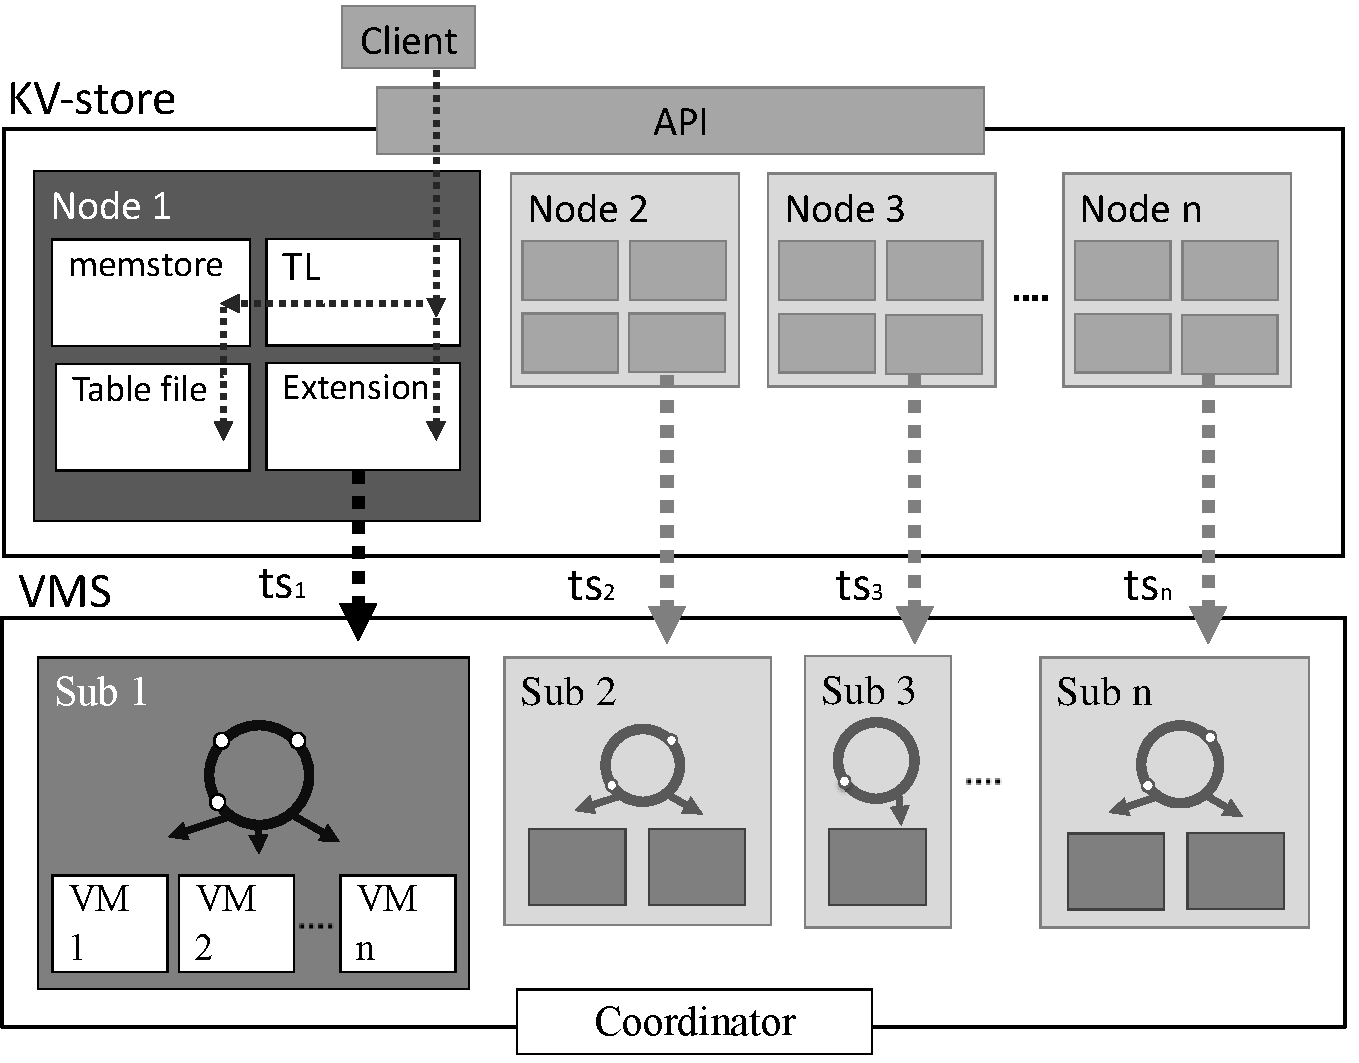
\includegraphics[width=0.7\linewidth]{figures/VMS_system_overview}
    	\label{fig:System_Design)}
    	\caption{System Design}
    \end{figure}
    
    \paragraph{Approach ---}
 	We describe and evaluate the design of a scalable view maintenance 
	system (VMS) \cite{Adler_2016_a}, that integrates with the widely used Apache HBase 
	KV-store, as it is shown on top of Figure~\ref{fig:System_Design)}. 
	As described before, the KV-store is an inherently
	distributed database. It runs a variable number of $n$ data nodes. The 
	incoming client request (i.e. the incoming data) are distributed over these 
	nodes. Node~1 in the figure depicts a magnification of the processes
	that are triggered during one client operation on a data node: the
	operation is written to a transaction log (TL), then it is inserted
	into a memstore and finally it is pushed to the table file on disk.
	The extension component is an additional component. It reads all new 
	client operations from the TL and forwards them to our VMS.   
	
 	On the bottom of the figure, the VMS is depicted. Queries can be issued 
	to the VMS in a SQL-like query language. The VMS, then, computes and 
	maintains the result of the queries in view tables (which are simple tables 
	in KV-store); its computations are based on a stream of client
	operations that it receives, in a distributed fashion (i.e. one stream 
	$ts$ per KV-node), from KV-store. The VMS, like KV-store, is a scalable 
	system. A variable number of $n$ sub systems, contain a variable number 
	of view managers (VMs) -- which are doing the actual work of computing and 
	applying the client operations to the view tables. 
		
	
 	The VMS offers an approach that scales in view update load and number 
	of views maintained. The design does not interfere with read/write 
	processing of tables in the KV-store, thus, leaving base table 
	processing latencies unaffected. It integrates "naturally" with 
	KV-store. Thus, our approach inherits the availability, reliability, and 
	scalability properties of KV-store itself. View tables can be split 
	across servers, distributed across the network, replicated across the 
	underlying file system, and made available to increasing number of 
	clients. 


	


    \begin{figure}[h]
    	\centering
    	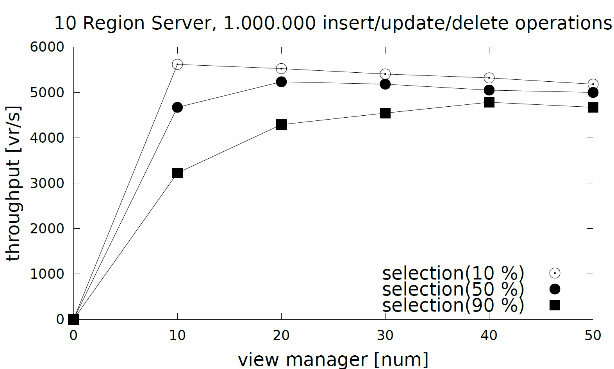
\includegraphics[width=0.7\linewidth]{figures/Effect_of_scaling_the_number_of_view_managers_for_selection_views}
    	\label{fig:scaling_VMs_selection_views}
    	\caption{Scaling the number of VMs for selection views}
    \end{figure}
    
    \begin{figure}[h]
     	\centering
     	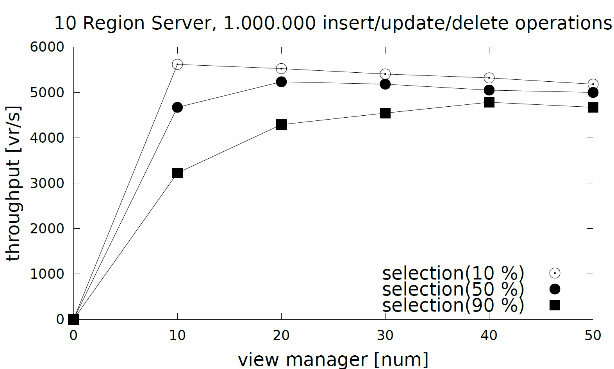
\includegraphics[width=0.7\linewidth]{figures/Effect_of_scaling_the_number_of_view_managers_for_selection_views}
     	\label{fig:scaling_VMs_aggregation_views}
     	\caption{Scaling the number of VMs for aggregation views}
     \end{figure}
     
     
    
   \paragraph{Implementation and results ---} 
 	We have implemented the VMS as a separate framework and integrated it 
	with Apache HBase (Version 0.98.1.6) \cite{Adler_2016_a}. The VMS has been 
	evaluated on a cluster of 40 nodes (cf. Fig. 
	\ref{fig:scaling_VMs_selection_views} \& 
	\ref{fig:scaling_VMs_aggregation_views}). We demonstrated that it is 
	possible to efficiently maintain the different view types (e.g., 
	selection, projection, aggregation and join views), as well as 
	combinations of complexer query constructions. The maintenance system is 
	horizontally scalable and achieves a maximum throughput on our cluster 
	of 6.000 view records per second. As the number of computed views grows, 
	more view manager processes can be deployed for the VMS; the VMS itself 
	adapts to varying load by performing an internal load balancing. 




     
   \paragraph{Next steps ---}
	 As next steps, we plan to investigate how to efficiently manage 
	multi-view processing, i.e., to share and reuse computations and reduce 
	the overall maintenance cost for the concurrent materialization of many 
	individual view expressions, which may even depend on one another. We
	build a model of $n$ directed acyclic graphs (i.e. DAGs), each 
	corresponding to the maintenance plan of one of our queries. Then, we 
	run an optimization algorithm, based on a cost model, to determine a
	global maintenance plan; the algorithm strives for sharing a maximum
	of intermediate results and reduces the global processing effort, as
	well as the overall storage cost.
	
	
	Also, we plan to investigate how to integrate our incremental view 
	maintenance approach with batch processing to enable the creation of new 
	view expressions on the fly, i.e., when existing base tables views depend 
	on are already available. 

  \paragraph{Publications ---}
	
   Jan Adler, Martin Jergler, Hans-Arno Jacobsen
   \textbf{Dynamic Scalable view maintenance in KV-stores}
   \textit{2016 USENIX Annual Technical Conference} (submitted for publication, March 2016).

  